\chapter{枚举与模式}\label{ch10}

\emph{Surprising how much computer stuff makes sense viewed as tragic deprivation of sum types (cf. deprivation of lambdas).}

\begin{flushright}
    ——Graydon Hoare
\end{flushright}

这一章的第一个话题将是一个古老的、强有力的、可以帮你在短期内完成很多工作的(有代价地)、并且在许多语言中以不同的名字广为人知的特性。但它并不是魔鬼。而是一种用户自定义的数据类型,它是ML和Haskell程序员们熟知的和类型、也是互斥的联合、还是代数数据类型。在Rust中,它们被称为\emph{枚举(enumerations)},或者简写为\emph{enum}。和魔鬼不同的是,它们非常安全、索取的代价也很小。

C++和C\#都有枚举,你可以使用它们来定义自己的类型,这种类型的取值范围是一些命名常量的集合。例如,你可能定义过一个叫\texttt{Color}的类型,取值范围为\texttt{Red}、\texttt{Orange}、\texttt{Yellow}等等。这种枚举在Rust中也能工作,但Rust进一步扩展了枚举。一个Rust枚举可以包含数据,包括多种不同类型的数据。例如,Rust的\texttt{Result<String, io::Error}类型是一个枚举;这样一个值要么是一个包含\texttt{String}的\texttt{Ok}值要么是一个包含\texttt{io::Error}的\texttt{Err}值。这就超出了C++和C\#中枚举的能力。它更像C中的\texttt{union}——但和联合不同的是,Rust的枚举是类型安全的。

枚举适用于一个值有多种可能的情况。使用它们的“代价”是你必须使用模式匹配来安全地访问数据,这也是我们这一章中的第二个话题。

如果你使用过Python的解包或者JavaScript中的解构,那你可能觉得模式也很熟悉,但Rust同样扩展了模式。Rust的模式有点像匹配数据的正则表达式。它们被用来测试一个值是否具有特定的期望的形态。它们可以一次从结构体或这元组中提取出多个字段存入局部变量。并且和正则表达式类似,它们很简洁,通常只用单行代码就能完成任务。

这一章将以枚举的基础开始,展示数据怎么被关联到枚举选项以及枚举是怎么存储在内存中的。然后我们会展示Rust的模式和\texttt{match}表达式如何简洁地指定基于枚举、结构体、数组、切片的逻辑。模式也可以包含引用、move和\texttt{if}条件,这让它们的功能更加强大。

\section{枚举}\label{enum}

简单的C风格枚举非常直观:
\begin{minted}{Rust}
    enum Ordering {
        Less,
        Equal,
        Greater,
    }
\end{minted}

这里声明了一个有三个可能的值的\texttt{Ordering}类型,这些值被称为\emph{variant}或者\emph{constructor}:\texttt{Ordering::Less}、\texttt{Ordering::Equal}、\texttt{Ordering::Greater}。这个枚举是标准库的一部分,因此Rust代码可以导入它:
\begin{minted}{Rust}
    use std::cmp::Ordering;

    fn compare(n: i32, m: i32) -> Ordering {
        if n < m {
            Ordering::Less
        } else if n > m {
            Ordering::Greater
        } else {
            Ordering::Equal
        }
    }
\end{minted}

或者它的所有constructor:
\begin{minted}{Rust}
    use std::cmp::Ordering::{self, *};  // `*`意思是导入所有的子item

    fn compare(n: i32, m: i32) -> Ordering {
        if n < m {
            Less
        } else if n > m {
            Greater
        } else {
            Equal
        }
    }
\end{minted}

导入constructor之后,我们可以写\texttt{Less}来代替\texttt{Ordering::Less}等,但因为这样不够明显,因此一般认为\emph{不要}导入它们式更好的风格,除非它能是你的代码的可读性更强。

为了导入一个在当前模块中声明的枚举的constructor,可以使用\texttt{self}:
\begin{minted}{Rust}
    enum Pet {
        Orca,
        Giraffe,
        ...
    }

    use self::Pet::*;
\end{minted}

在内存中,C风格的枚举值被存储为整数。有时告诉Rust使用哪些整数会很有用:
\begin{minted}{Rust}
    enum HttpStatus {
        Ok = 200,
        NotModified = 304,
        NotFound = 404,
        ...
    }
\end{minted}

否则,Rust会从0开始自动分配值。

默认情况下,Rust用能容纳所有值的最小的内建整数类型来存储C风格枚举。大多数情况下都是一个单独的字节:
\begin{minted}{Rust}
    use std::mem::size_of;
    assert_eq!(size_of::<Ordering>(), 1);
    assert_eq!(size_of::<HttpStatus>(), 2); // 404不能存储在u8中
\end{minted}

你可以通过添加\texttt{\#[repr]}属性来覆盖Rust选择的内存表示方式。更多的细节见“\nameref{repr}”。

将C风格的枚举转换为整数是允许的:
\begin{minted}{Rust}
    assert_eq!(HttpStatus::Ok as i32, 200);
\end{minted}

然而,反过来把整数转换为枚举是不允许的。和C和C++不同,Rust保证枚举的值只能是\texttt{enum}生命中列出的值之一。未经检查的从整数类型到枚举类型的转换会打破这种保证,所以它是不允许的。你可以写出你自己的带检查的版本:
\begin{minted}{Rust}
    fn http_status_from_u32(n: u32) -> Option<HttpStatus> {
        match n {
            200 => Some(HttpStatus::Ok),
            304 => Some(HttpStatus::NotModified),
            404 => Some(HttpStatus::NotFound),
            ...
            _ => None,
        }
    }
\end{minted}

或者使用\href{https://crates.io/crates/enum_primitive}{\texttt{enum\_primitive}} crate。它包含一个宏可以为你自动生成这种类型的转换代码。

和结构体一样,编译器也可以为你自动生成类似\texttt{==}运算符这样的特性,但你需要显式地要求这样:
\begin{minted}{Rust}
    #[derive(Copy, Clone, Debug, PartialEq, Eq)]
    enum TimeUnit {
        Seconds, Minutes, Hours, Days, Months, Years,
    }
\end{minted}

枚举也和结构体一样可以拥有方法:
\begin{minted}{Rust}
    impl TimeUnit {
        /// 返回该时间单位的复数名词。
        fn plural(self) -> &'static str {
            match self {
                TimeUnit::Seconds => "seconds",
                TimeUnit::Minutes => "minutes",
                TimeUnit::Hours => "hours",
                TimeUnit::Days => "days",
                TimeUnit::Months => "months",
                TimeUnit::Years => "years",
            }
        }

        /// 返回该时间单位的单数名词。
        fn singular(self) -> &'static str {
            self.plural().trim_end_matches('s')
        }
    }
\end{minted}

C风格的枚举就这么多内容了。Rust中最有趣的一类枚举是那些带有数据的枚举。我们将展示这些枚举如何存储在内存中、如何通过添加类型参数将它们变为泛型的,以及如何通过枚举构建复杂的数据结构。

\subsection{带有数据的枚举}

一些程序总是需要显示完整的日期和时间,并且精确到毫秒。但对于大多数程序,显示大概的时间范围会更加友好,例如“两个月以前”。我们可以用之前定义的枚举编写一个新的枚举来实现这一点:
\begin{minted}{Rust}
    /// 一个故意舍入的时间戳,因此我们的程序会显示“6个月以前”
    /// 而不是“February 9, 2016, at 9:49 AM”。
    #[derive(Copy, Clone, Debug, PartialEq)]
    enum RoughTime {
        InThePast(TimeUnit, u32),
        JustNow,
        InTheFuture(TimeUnit, u32),
    }
\end{minted}

这个枚举中的两个variant,即\texttt{InThePast}和\texttt{InTheFuture}都有参数。这些被称为\emph{tuple variant}。就像类元组结构体一样,它们的constructor是创建新的\texttt{RoughTime}值的函数:
\begin{minted}{Rust}
    let four_score_and_seven_years_ago =
        RoughTime::InThePast(TimeUnit::Years, 4 * 20 + 7);

    let three_hours_from_now =
        RoughTime::InTheFuture(TimeUnit::Hours, 3);
\end{minted}

枚举也可以有\emph{struct variant},它们和普通的结构体一样拥有命名字段:
\begin{minted}{Rust}
    enum Shape {
        Sphere { center: Point3d, radius: f32 },
        Cuboid { corner1: Point3d, corner2: Point3d },
    }

    let unit_sphere = Shape::Sphere {
        center: ORIGIN,
        radius: 1.0,
    };
\end{minted}

总的来说,Rust有三种枚举variant,分别对应我们在上一章中展示的三种结构体。没有数据的variant对应类单元结构体。元组variant对应类元组结构体。结构体variant对应有花括号和命名字段的结构体。一个枚举可以同时有这三种variant:
\begin{minted}{Rust}
    enum RelationshipStatus {
        Single,
        InARelationship,
        ItsComplicated(Option<String>),
        ItsExtremelyComplicated {
            car: DifferentialEquation, 
            cdr: EarlyModernistPoem,
        },
    }
\end{minted}

所有种类的constructor都和枚举自身有相同的可见性。

\subsection{内存中的枚举}

在内存中,带有数据的枚举被存储为一个很小的整数\emph{标签(tag)},加上一块足够存储所有variant中最大的那个的内存。标签字段是Rust内部要使用的,它表示是哪一个constructor创建了这个值,进而得知这个值有哪些字段。

在Rust 1.50中,\texttt{RoughTime}存储为8个字节,如\hyperref[f10-1]{图10-1}所示。

\begin{figure}[htbp]
    \centering
    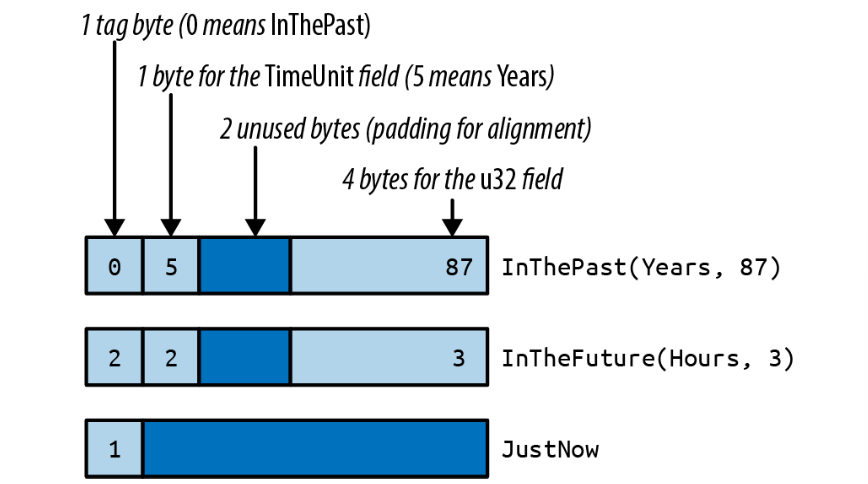
\includegraphics[width=0.9\textwidth]{../img/f10-1.png}
    \caption{内存中的\texttt{RoughTime}值}
    \label{f10-1}
\end{figure}

对于枚举的布局Rust不做任何保证。然而,为了给将来的优化留下余地,在一些情况下它可能会用比图中所示更加高效的方式包装一个枚举。例如,一些泛型结构体可以不用标签存储,我们稍后会讲到它。

\subsection{使用枚举实现富数据结构}

枚举在实现树形结构时也很有用。例如,假设一个Rust程序要处理任意的Json数据。在内存中,任何Json文档都可以被表示为一个这种Rust类型的值:
\begin{minted}{Rust}
    use std::collections::HashMap;

    enum Json {
        Null,
        Boolean(bool),
        Number(f64),
        String(String),
        Array(Vec<Json>),
        Object(Box<HashMap<String, Json>>),
    }
\end{minted}

与Rust代码相比,用英文来解释这个数据结构也不会再有太大的改进了。JSON标准定义了可以出现在JSON文档中的数据类型:\texttt{null}、布尔值、数字、字符串、JSON值的数组、以及带有字符串键和JSON值的对象。这个\texttt{Json}枚举简单地列出了这些类型。

这并不是一个假想的例子。你可以在\texttt{serde\_json} crate中找到一个非常相似的枚举,它是一个用于Rust结构体序列化的库,也是crates.io上下载次数最多的crate之一。

用于表示\texttt{Object}的\texttt{HashMap}外层的\texttt{Box}只是为了让\texttt{Json}值更加紧凑。在内存中,\texttt{Json}类型的值将占据4个机器字。\texttt{String}和\texttt{Vec}都是3个字,Rust会再添加一个字节的标签,再加上对齐所以总共是4个字。\texttt{Null}和\texttt{Boolean}值没有足够的数据利用全部的空间,但所有的\texttt{Json}值大小必须相同,因此这时多余的空间就被浪费了。\hyperref[f10-2]{图10-2}展示了一些示例的\texttt{Json}值在内存中的实际视图。

\begin{figure}[htbp]
    \centering
    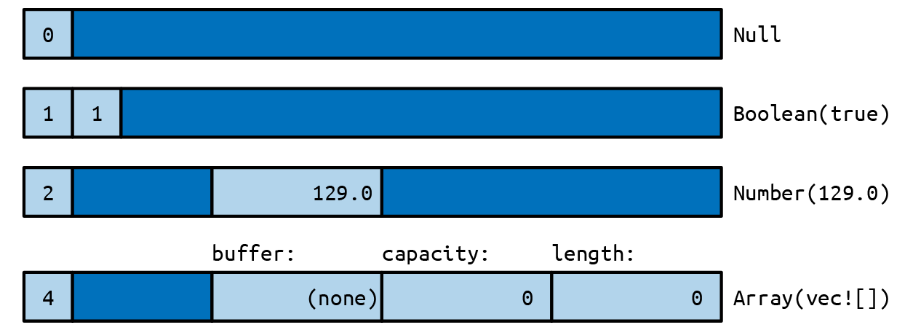
\includegraphics[width=0.8\textwidth]{../img/f10-2.png}
    \caption{内存中的\texttt{Json}值}
    \label{f10-2}
\end{figure}

一个\texttt{HashMap}会更大如果我们一定要在每一个\texttt{Json}值中给它留出空间,它们将会变得更大,也就是8个字。但\texttt{Box<HashMap>}是单个字:它只是一个指向堆上分配的数据的指针。我们甚至可以通过装箱更多的字段来让\texttt{Json}变得更加紧凑。

这里优秀的地方在于,我们如此简单的就完成了这一切。如果是在C++中,可能要写一个这样的一个类才行:
\begin{minted}{Rust}
    class JSON {
    private:
        enum Tag {
            Null, Boolean, Number, String, Array, Object
        };
        union Data {
            bool boolean;
            double number;
            shared_ptr<string> str;
            shared_ptr<vector<JSON>> array;
            shared_ptr<unordered_map<string, JSON>> object;

            Data() {}
            ~Data() {}
            ...
        };
        
        Tag tag;
        Data data;
    
    public:
        bool is_null() const { return tag == Null; }
        bool is_boolean const { return tag == Boolean; }
        bool get_boolean() const {
            assert(is_boolean());
            return data.boolean;
        }
        void set_boolean(bool value) {
            this->~JSON();  // 清除string/array/object值
            tag = Boolean;
            data.boolean = value;
        }
        ...
    };
\end{minted}

30行代码,我们才刚刚开始。这个类还需要构造函数、析构函数、一个赋值运算符。另一种方案是通过继承,首先创建一个基类\texttt{JSON}和它的子类\texttt{JSONBoolean}、\texttt{JSONString}等等。无论哪种方式,等到完成之后,我们的C++ JSON库都要有一堆代码了。其他程序员需要花费不少精力来阅读和使用它。而Rust的整个枚举只需要8行代码。

\subsection{泛型枚举}
枚举可以是泛型的。标准库的两个例子几乎是整个语言中使用最广泛的数据类型:
\begin{minted}{Rust}
    enum Option<T> {
        None,
        Some(T),
    }

    enum Result<T, E> {
        Ok(T),
        Err(E),
    }
\end{minted}

到现在这些类型你应该已经很熟悉了,泛型枚举的语法和泛型结构体完全相同。

一个不明显的细节是当类型\texttt{T}是引用、\texttt{Box}或其他智能指针类型时Rust可以省略\texttt{Option<T>}的标签字段。因为这些指针类型中的任何一个都不允许为0,所以Rust可以用单个机器字来表示\texttt{Option<Box<i32>>}:用0表示\texttt{None},用非0表示\texttt{Some}指针。这使得这样的\texttt{Option}类型与C和C++中可以为空的指针值非常相似。不同之处在于Rust的类型系统要求你必须先检查\texttt{Option}的值是\texttt{Some},然后才能使用它内含的值。这有效的避免了空指针解引用。

泛型数据结构体可以用很少的几行代码构建:
\begin{minted}{Rust}
    // 一个`T`类型的有序集合
    enum BinaryTree<T> {
        Empty,
        NonEmpty(Box<TreeNode<T>>),
    }

    // 二叉树的一部分
    struct TreeNode<T> {
        element: T,
        left: BinaryTree<T>,
        right: BinaryTree<T>,
    }
\end{minted}

这几行代码定义了一个可以存储任意数量的\texttt{T}类型值的\texttt{BinaryTree}类型。

这两个定义包含了大量信息,所以我们将花费一些时间把代码翻译为中文。每一个\texttt{BinaryTree}值是\texttt{Empty}或者\texttt{NonEmpty}。如果它是\texttt{Empty},那么它不包含任何数据。如果是\texttt{NonEmpty},那么它会包含一个\texttt{Box},这个指针指向一个在堆上分配的\texttt{TreeNode}值。

每一个\texttt{TreeNode}值包含一个实际的元素,和两个\texttt{BinaryTree}值。这意味着一棵树可以包含子树,因此一个\texttt{NonEmpty}树可以包含任意数量的后台节点。

一个\texttt{BinaryTree<\&str>}类型的值的视图如\hyperref[f10-3]{图10-3}所示。因为对于\texttt{Option<Box<T>>},Rust会省略标签字段,所以一个\texttt{BinaryTree}值只占一个机器字。

\begin{figure}[htbp]
    \centering
    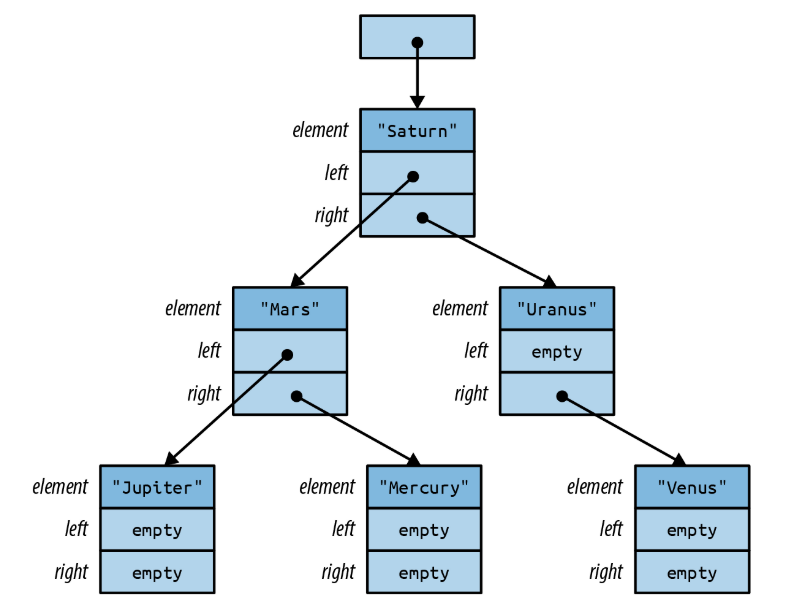
\includegraphics[width=0.9\textwidth]{../img/f10-3.png}
    \caption{一个包含6个字符串的\texttt{BinaryTree}}
    \label{f10-3}
\end{figure}

构建这棵树中的节点非常直观:
\begin{minted}{Rust}
    use self::BinaryTree::*;
    let jupiter_tree = NonEmpty(Box::new(TreeNode {
        element: "Jupiter",
        left: Empty,
        right: Empty,
    }));
\end{minted}

更大的树可以通过较小的树构建:
\begin{minted}{Rust}
    let mars_tree = NonEmpty(BOx::new(TreeNode {
        element: "Mars",
        left: jupiter_tree,
        right: mercury_tree,
    }));
\end{minted}

自然地,这个赋值会把\texttt{jupiter\_node}和\texttt{mercury\_node}的所有权移动到新的父节点里。

树的其他部分遵循相同的模式。根节点和其它节点不同:
\begin{minted}{Rust}
    let tree = NonEmpty(Box::new(TreeNode {
        element: "Saturn",
        left: mars_tree,
        right: uranus_tree,
    }));
\end{minted}

在这一章的后续部分中,我们将介绍怎么在\texttt{BinaryTree}类型上实现一个\texttt{add}方法,这样我们就可以这样写:
\begin{minted}{Rust}
    let mut tree = BinaryTree::Empty;
    for planet in planets {
        tree.add(planet);
    }
\end{minted}

无论你之前用什么语言,在Rust中创建像\texttt{BinaryTree}这样的数据结构都需要一些练习。一开始把\texttt{Box}放在哪可能并不明显。一种寻找设计的方法是画一幅像\hyperref[f10-3]{图10-3}这样的内存布局图。然后根据图设计代码:每一个矩形都是一个结构体或者元组,每一个箭头都是一个\texttt{Box}或者其他智能指针。搞清楚每个字段的类型有点困难,但解决难题的回报是控制程序的内存使用。 

现在就到了我们在本章开始时提到的“代价”。枚举的标签字段要占用很小的内存,最糟的情况下要占用8个字节,但这种情况通常非常少见。枚举真正的缺点(如果它能被称为缺点的话)是Rust不能忽略安全性、不管当前的值是什么直接尝试访问字段:
\begin{minted}{Rust}
    let r = shape.radius;   // 错误:`Shape`类型没有字段`radius`
\end{minted}

访问枚举中的值的唯一方式是:使用枚举,这是一种安全的方式。

\section{模式}
